\appendix
% the appendix command just changes heading styles for appendices.

\chapter{System and software environment}

\section{ABC SMC implementation}

\subsection{Local machine}

Local development machine is a Mac laptop, running on macOS 10.15.6. The environment of the development is listed in Table \ref{table:local_macine}.

\begin{table}[H]
    \centering
    \begin{tabular}{|c c|}
        \hline
        Environment        & Version                \\ [0.5ex]
        \hline\hline
        Operating system   & macOS Catalina 10.15.6 \\
        PyCharm (IDE)      & Professional 202.2     \\
        Python interpretor & 3.7.0                  \\
        IPython            & 7.12.0                 \\
        Clang              & 6.0 (clang-600.0.57)   \\
        \hline
    \end{tabular}
    \caption{Environment on local machine}
    \label{table:local_macine}
\end{table}

Version requirements for some critical site packages (\verb|Python|) used in the code are listed in Table \ref{table:local_package}.

\begin{table}
    \centering
    \begin{tabular}{|c c|}
        \hline
        Environment & Version         \\ [0.5ex]
        \hline\hline
        pyABC       & $\simeq$ 0.10.3 \\
        NumPy       & $\simeq$ 1.18.4 \\
        SciPy       & $\simeq$ 1.4.1  \\
        pandas      & $\simeq$ 1.1.0  \\
        matplotlib  & $\simeq$ 3.0.1  \\
        bokeh       & $=$ 1.4.0       \\
        \hline
    \end{tabular}
    \caption{Site packages on local machine}
    \label{table:local_package}
\end{table}

Local development and some runs of small size were done under the hardware listed in Table \ref{table:local_hardware}. When running ABC SMC, the program can make used of 8 python process (Hyper-Threading enabled) and run under 3.8GHz (maximal) for a long time under proper cooling, proved that the program could efficiently use the computation resources for a local personal computer. It is noted that the program took no advantage of graphics card, as \verb|multiprocessing| along can only exploit the resources inside CPU. The execution time and other performance data presented in Chapter 5 were obtained using remote machines but not local machine.

\begin{table}
    \centering
    \begin{tabular}{|c c|}
        \hline
        Hardware        & Detail                                \\ [0.5ex]
        \hline\hline
        CPU             & Quad-Core Intel Core i5 8259U 2.3 GHz \\
        Architecture    & 64 Bit                                \\
        Hyper-Threading & Supported                             \\
        Turbo Boost     & Max 3.8 GHz                           \\
        Memory          & 16 GB                                 \\
        Graphics card   & Iris Plus Graphics 655                \\
        \hline
    \end{tabular}
    \caption{Hardwares on local machine}
    \label{table:local_hardware}
\end{table}



\subsection{Remote machine}

Cirrus hardware can be found in \url{https://www.cirrus.ac.uk/about/hardware.html}. The software environment used in the development and experiments are listed in Table \ref{table:cirrus_soft}. Requirement of site packages is the sanme as that on local macine (Table \ref{table:local_package})  

\begin{table}[H]
    \centering
    \begin{tabular}{|c c|}
        \hline
        Environment           & Version                      \\ [0.5ex]
        \hline\hline
        Operating system      & Red Hat Enterprise Linux 8.1 \\
        miniconda environment & 4.8.3                        \\
        Python interpreter    & 3.7.7                        \\
        gcc                   & 6.3.0                        \\
        \hline
    \end{tabular}
    \caption{Environment on local machine}
    \label{table:cirrus_soft}
\end{table}

% \section{Data analysis}

\chapter{Data and supplementary figures}






\section{Infer-back experiments}

\subsection{Parameter values used to generate synthetic data}

\begin{table}[H]
    \centering
    \begin{tabular}{|c c|}
        \hline
        Parameter            & Value \\[0.5ex]
        \hline\hline
        $\lambda_N$          & 2.20  \\
        $\kappa_{N\beta}$    & 3.96  \\
        $\mu_N$              & 1.72  \\
        $\nu_{N\Phi}$        & 0.219 \\
        \hline
        $\lambda_\Phi$       & 1.31  \\
        $\kappa_{\Phi\beta}$ & 0.124 \\
        $\mu_\Phi$           & 0.145 \\
        \hline
        $s_{\beta N}$        & 6.55  \\
        $i_{\beta\Phi}$      & 1.71  \\
        $\mu_\beta$          & 0.521 \\
        \hline
        $s_{\alpha\Phi}$     & 10.2  \\
        $\mu_\alpha$         & 19.7  \\
        \hline
    \end{tabular}
    \caption[Parameter values used to generate synthetic data for model 1]
    {Parameter values used to generate synthetic data for model 1. They were obtained from a preliminarily least-square fitting}
    \label{table:known_values}
\end{table}

\subsection{Kernel experiment: median epsilon schedule}

\begin{figure}[H]

    \begin{center}
        \resizebox{1.0\hsize}{!}{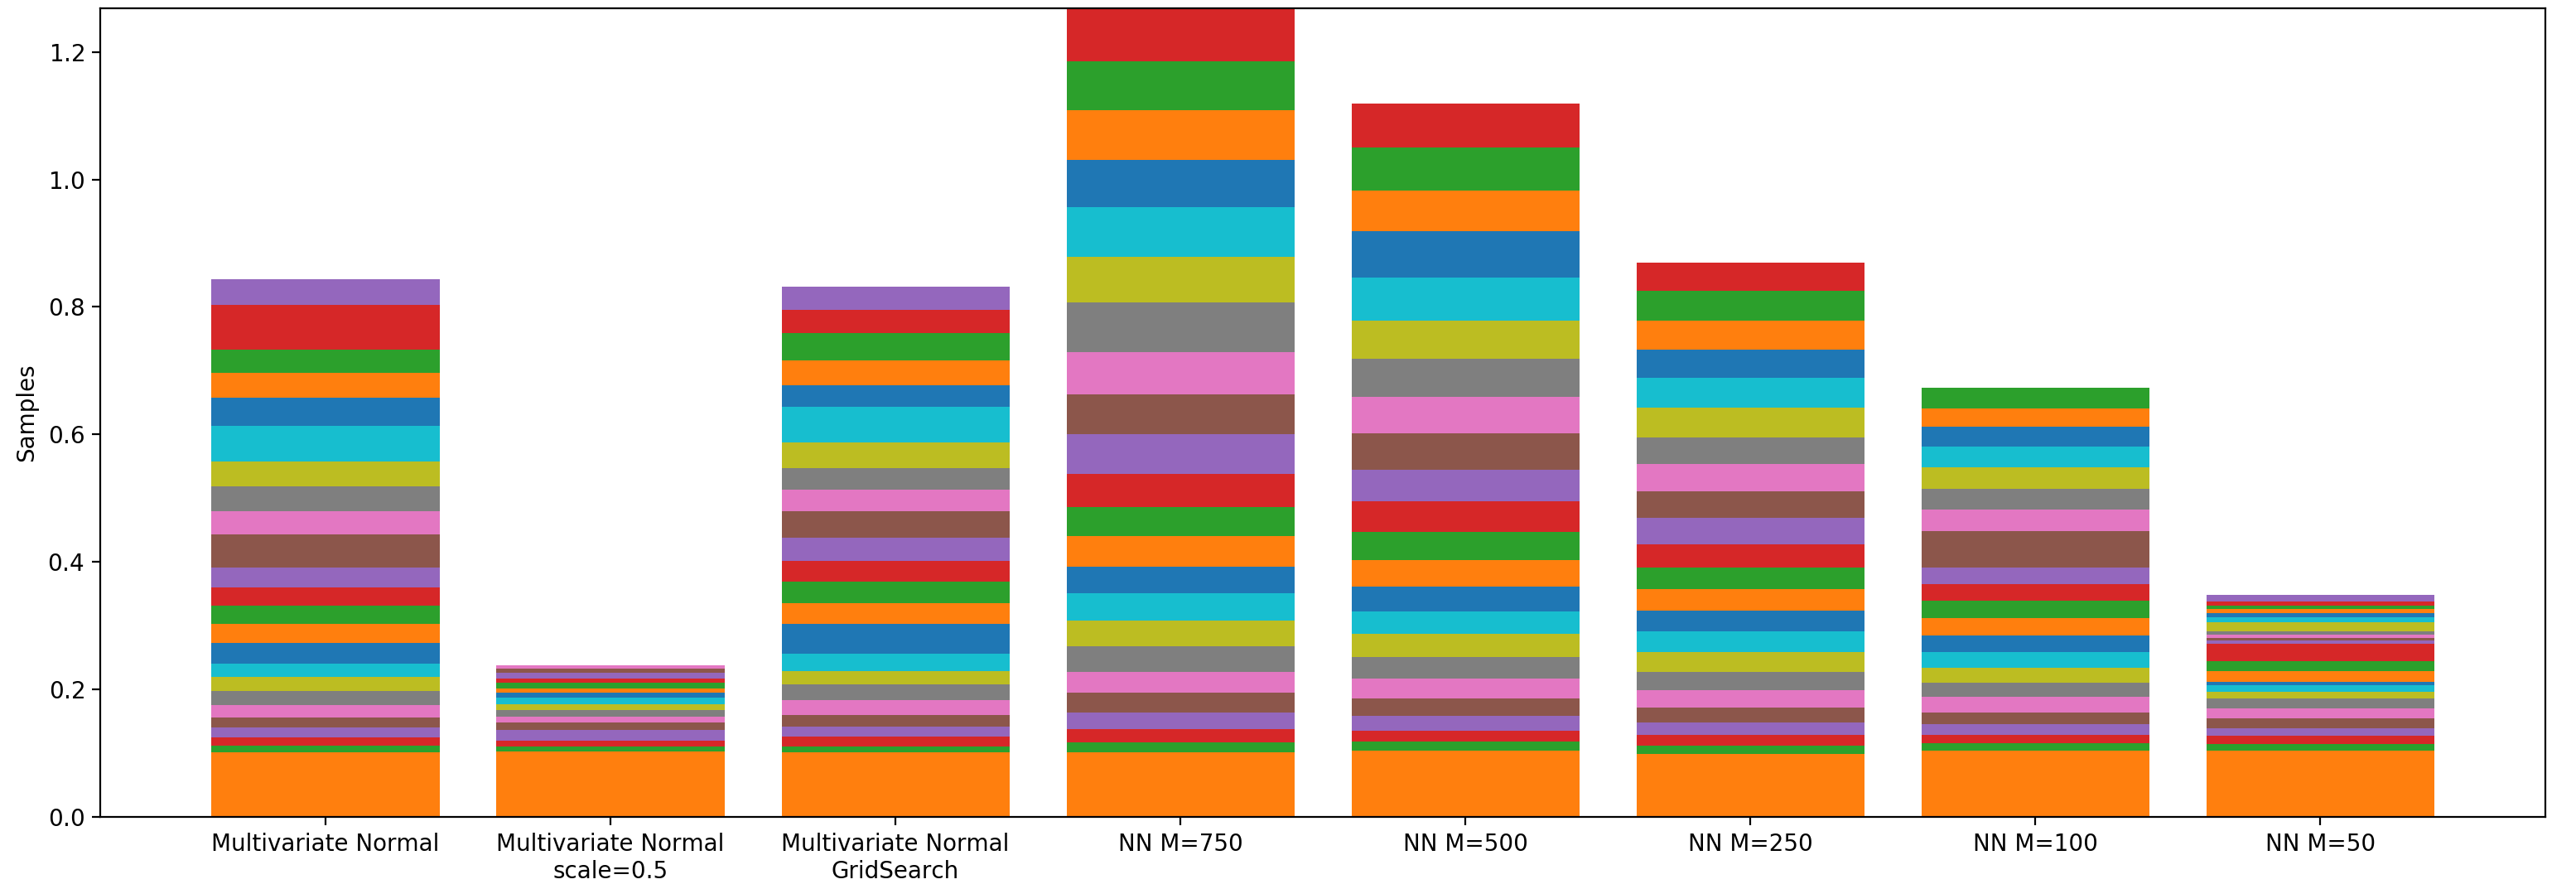
\includegraphics{fig/kernel2.png}}
    \end{center}

    \caption[Total sampling size of different kernels, using median epsilon strategy]
    {Total sampling size of different kernels, using median epsilon strategy. Different color represents different generations (bottom to top: population 1 to population 20)}
    \label{fig:kernel2}

    \begin{center}
        \resizebox{1.0\hsize}{!}{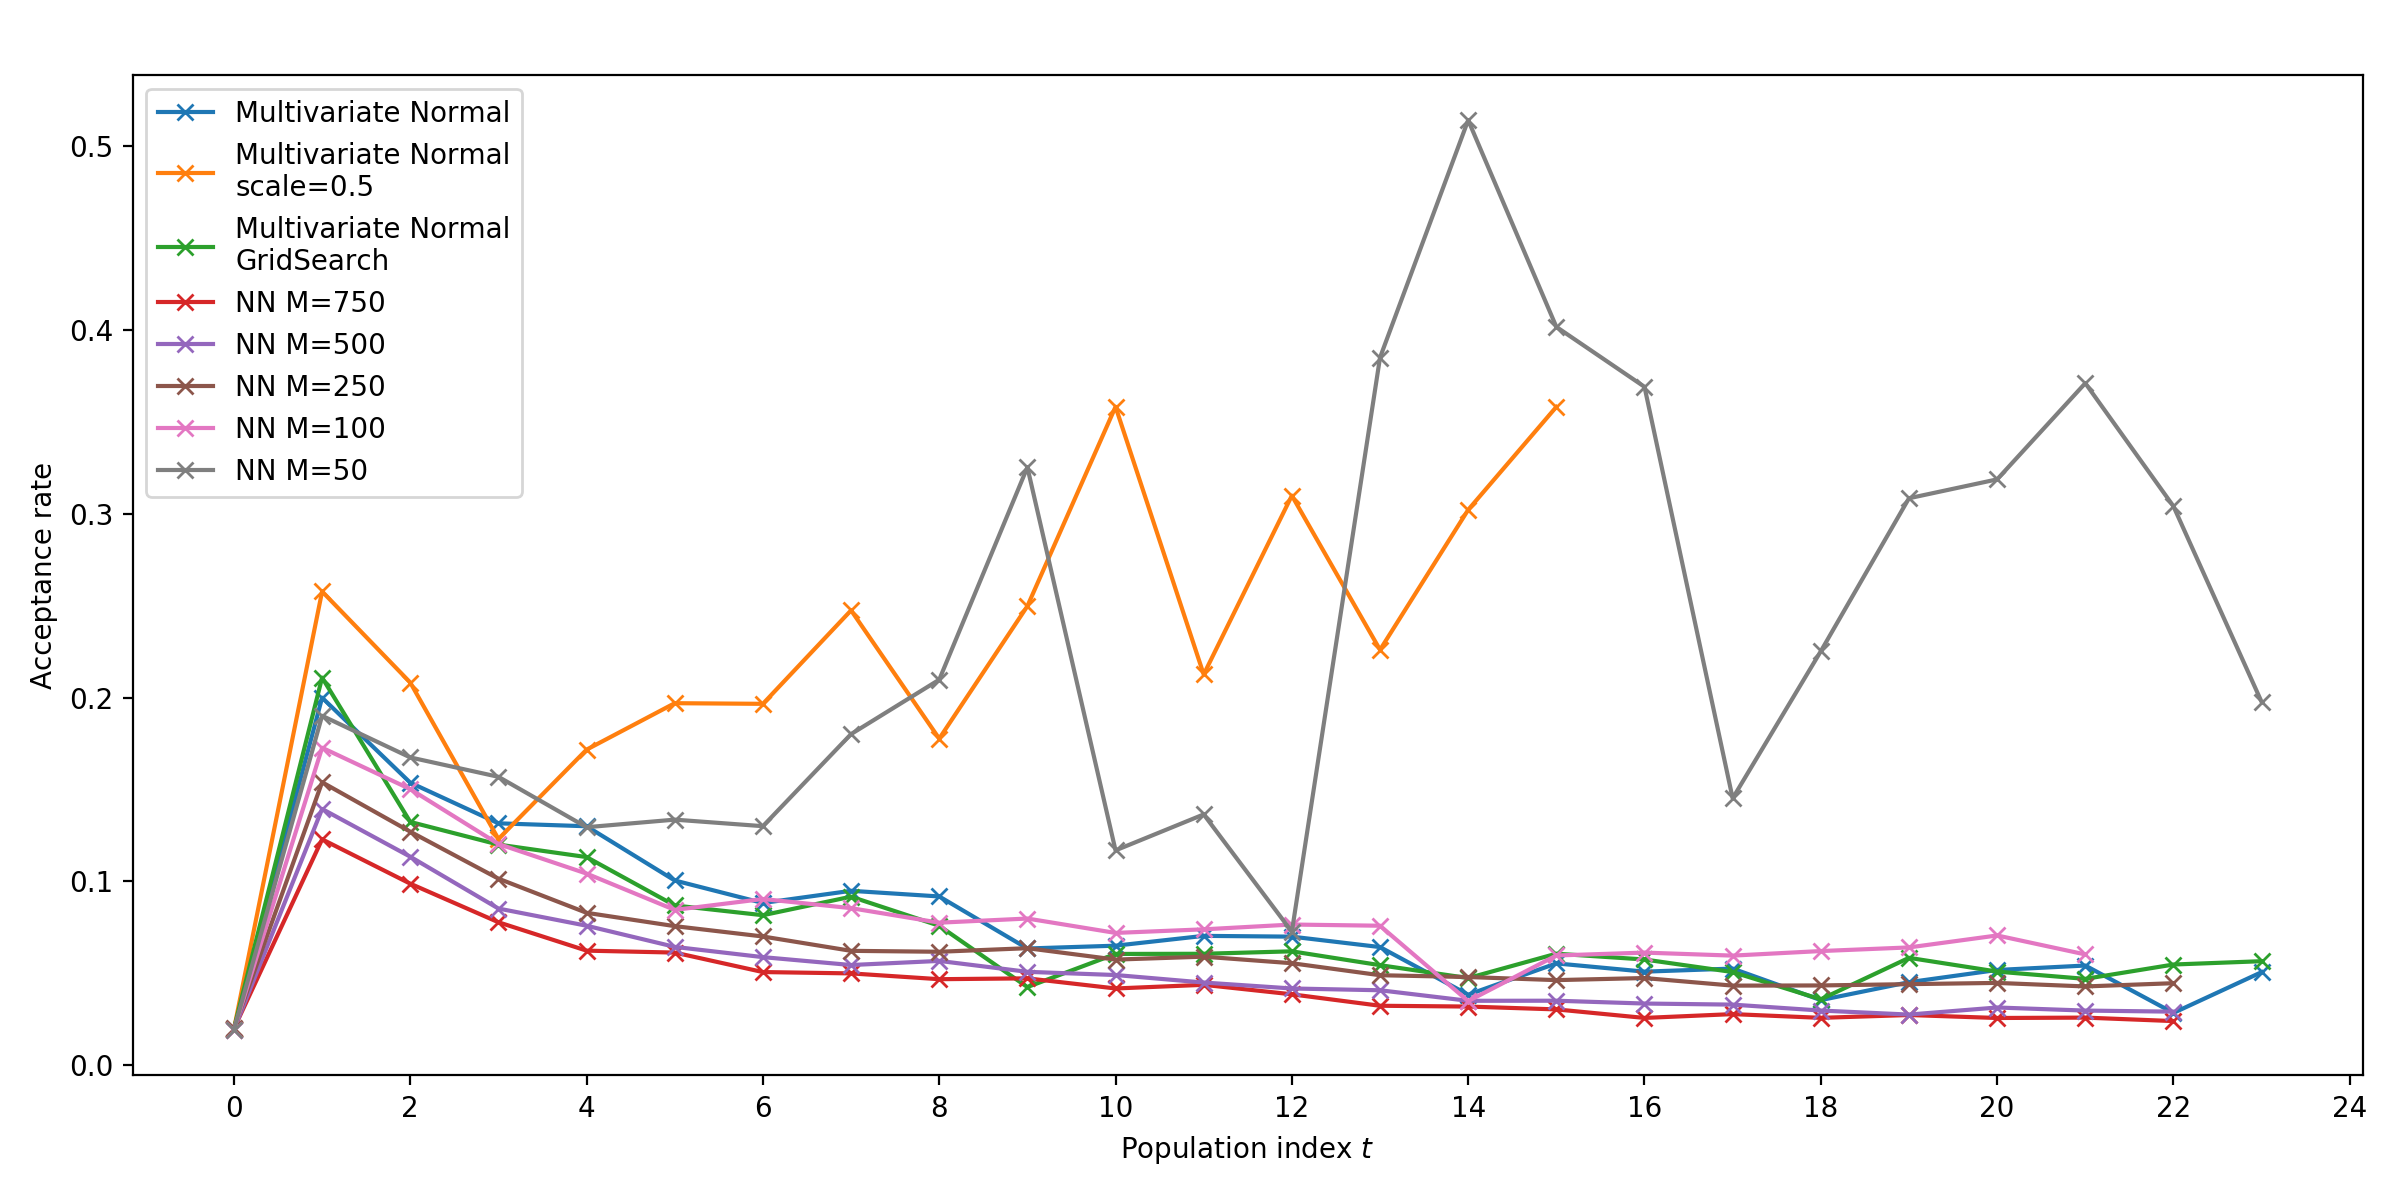
\includegraphics{fig/acceptance2.png}}
    \end{center}

    \caption[Acceptance rates of different kernels, using median epsilon strategy]
    {Acceptance rates of different kernels, using median epsilon strategy. Each population has 2000 particles. The total length of populations is different because some runs reached the final $\epsilon_T$ earlier than others}
    \label{fig:acceptance2}

\end{figure}


\section{Parameter inference and model comparison results}

\begin{figure}[H]

    \begin{center}
        \resizebox{1.0\hsize}{!}{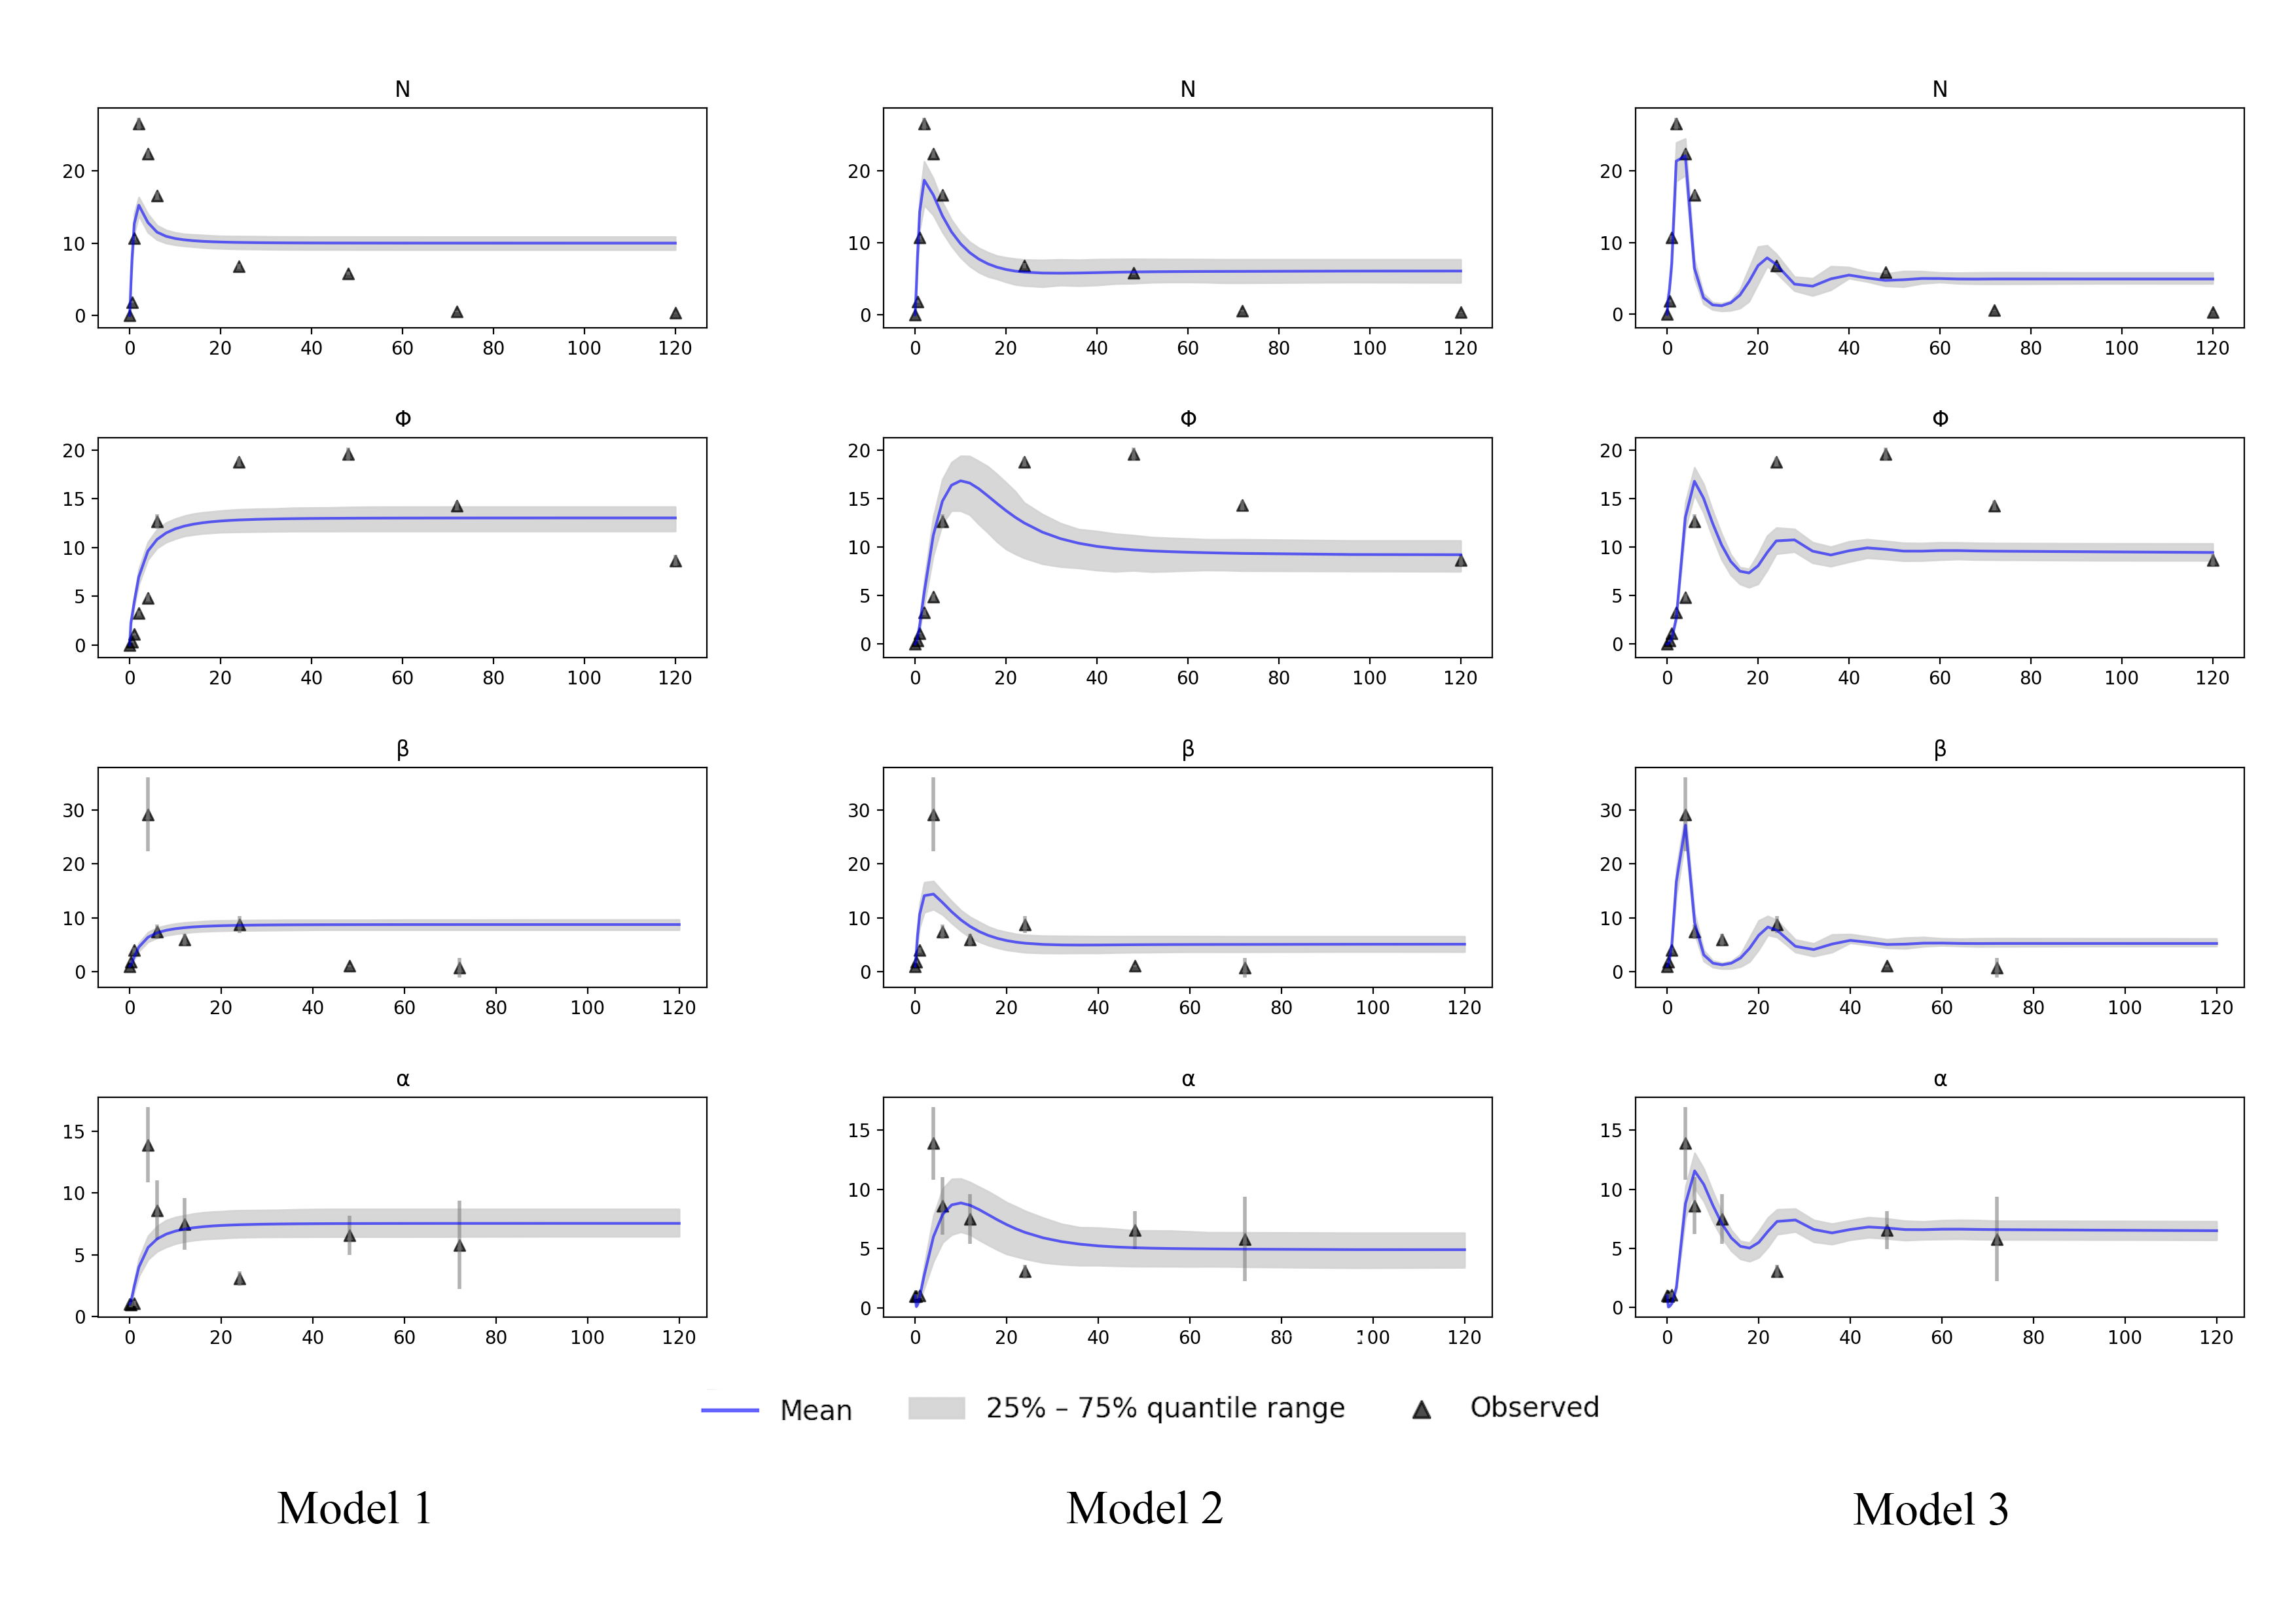
\includegraphics{fig/resultCurve_uni.png}}
    \end{center}

    \caption[Simulated data from the last population of model 1, 2 and 3, using uniform prior]{Simulated data from the last population of model 1, 2 and 3, using uniform prior.  Error bar indicates SEM (for $N$ and $\Phi$ the SEM is relatively small)}
    \label{fig:resultCurve_uni}


\end{figure}

\begin{figure}[ht]
    \begin{center}
        \resizebox{1.0\hsize}{!}{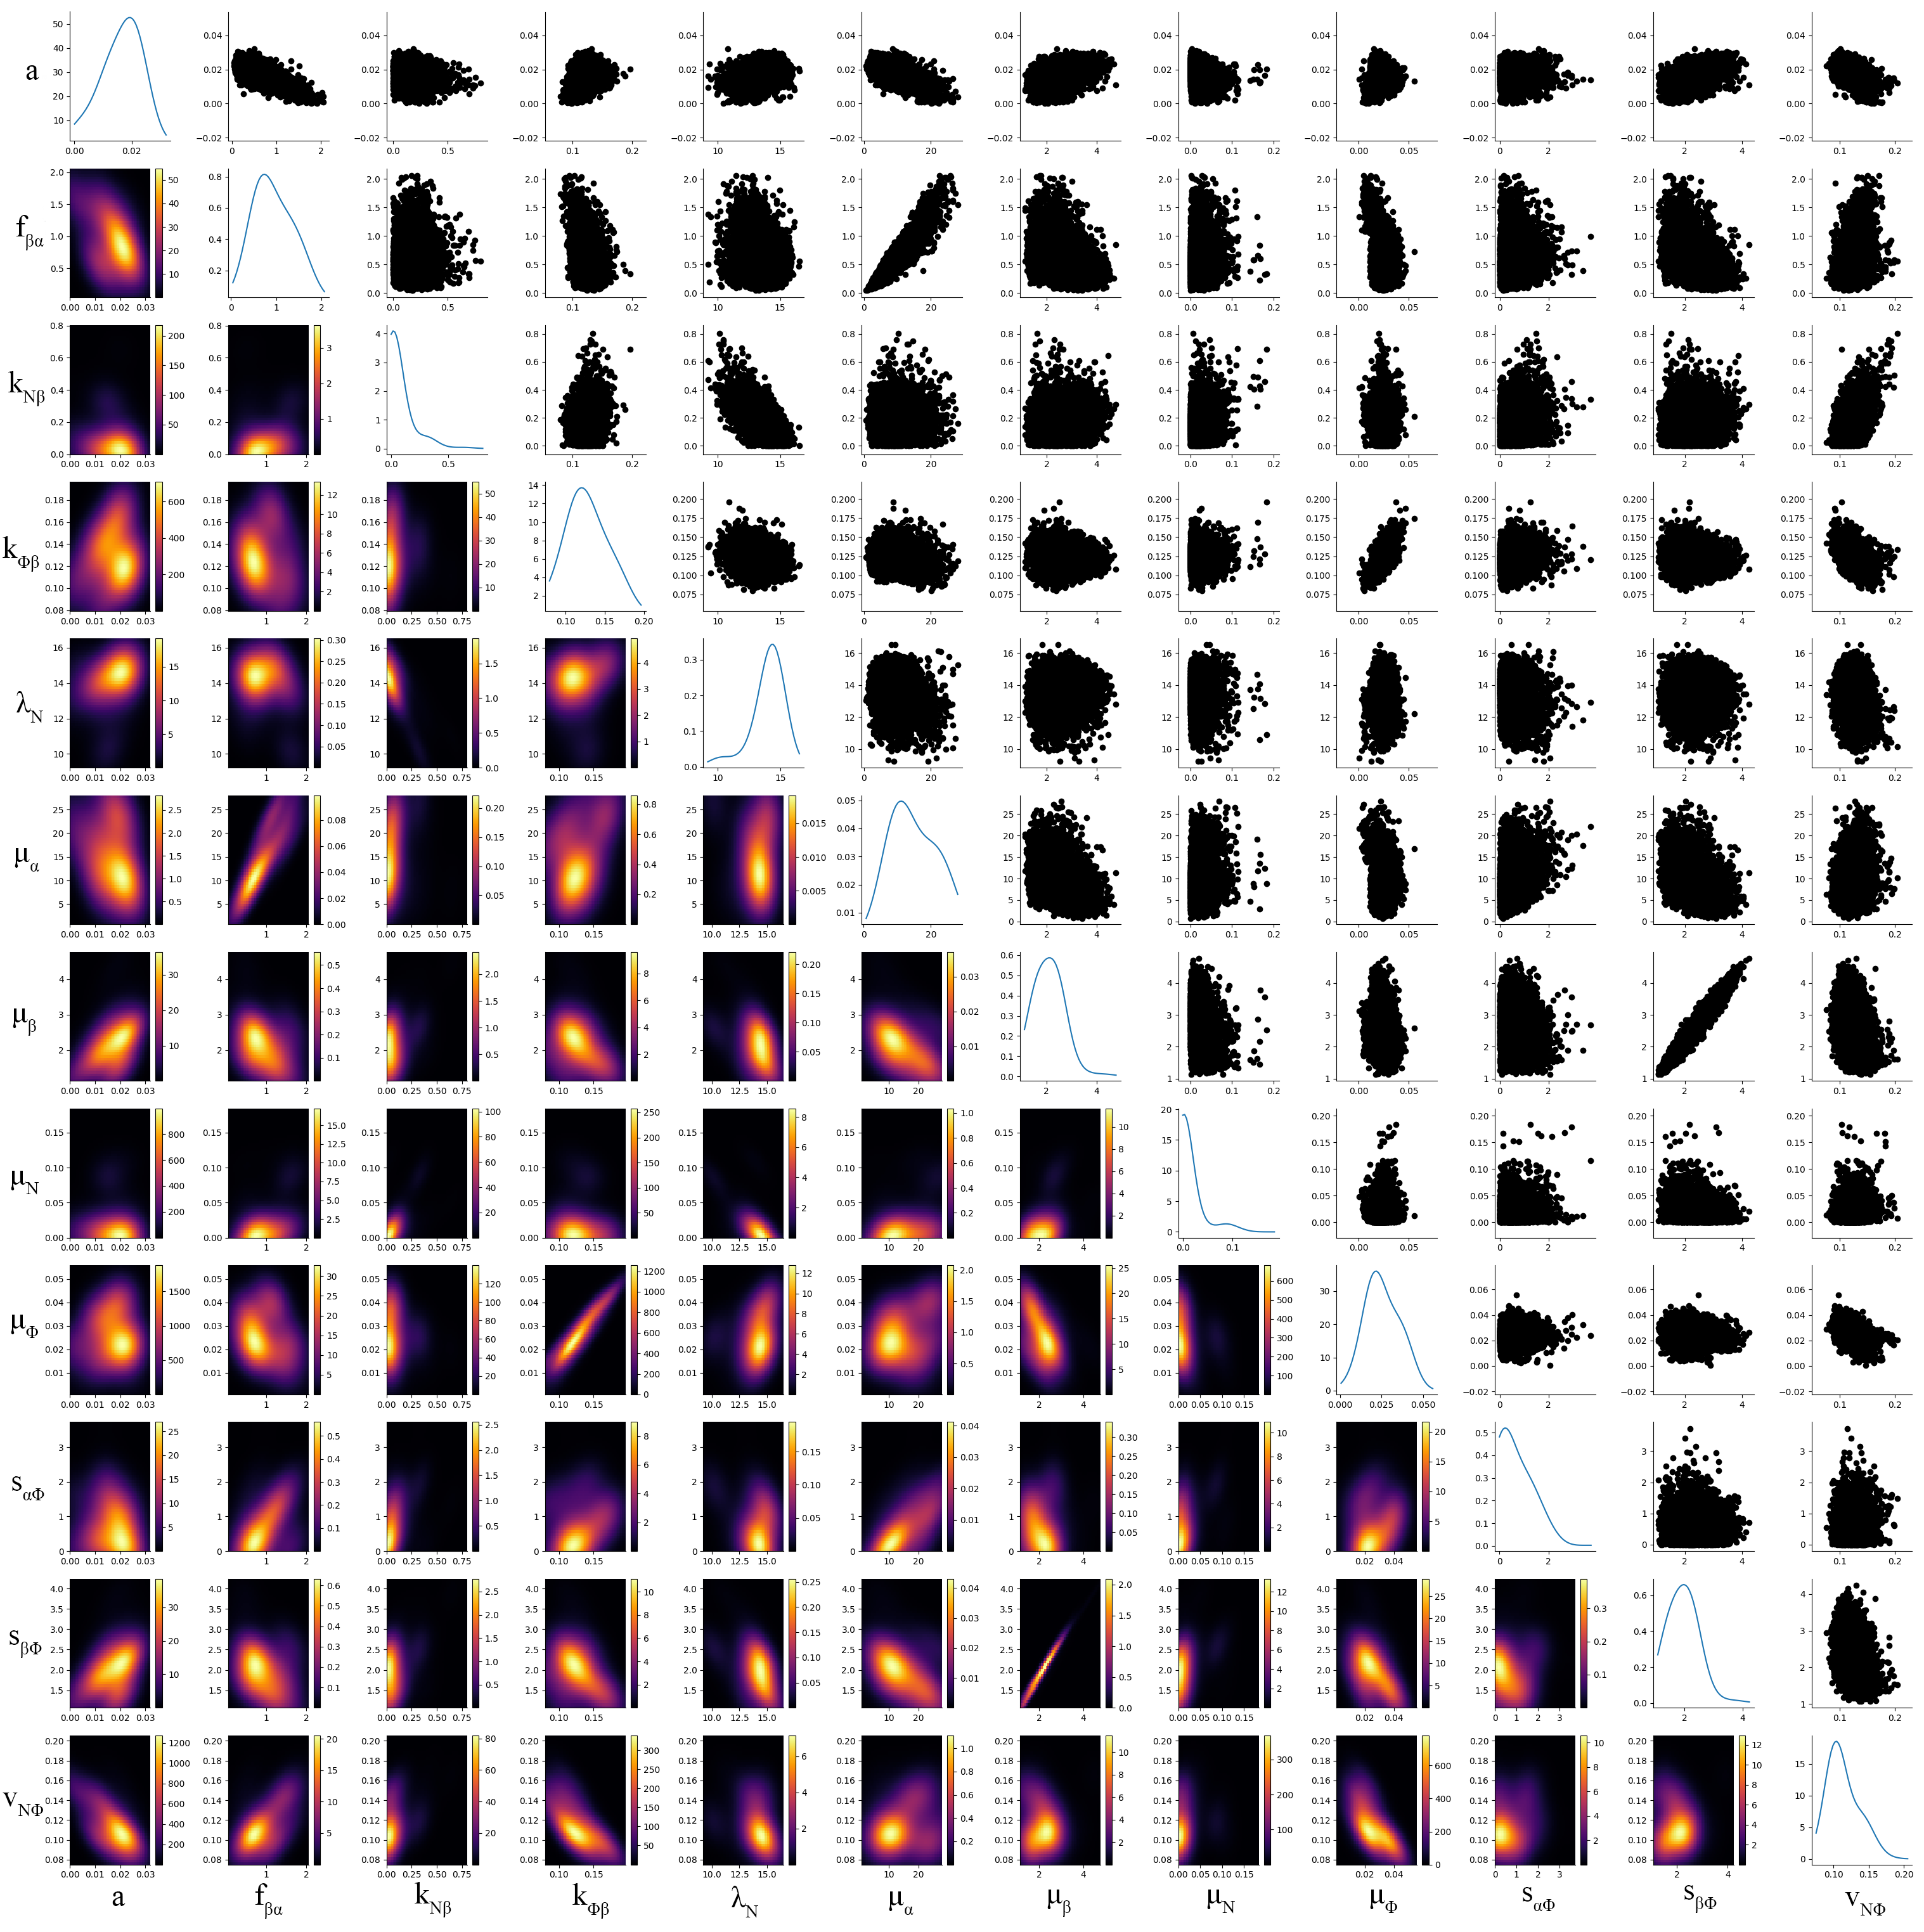
\includegraphics{fig/inferno5.png}}
    \end{center}
    \caption[Joint density distribution of each parameter pair]%
    {Joint distribution of each parameter pair. The diagonal is KDE fit of each individual parameter, the upper triangle contains scatter plot of the particles and the lower triangle is the joint density distribution for each parameter pair}
    \label{fig:model5_para_joint}
\end{figure}

\begin{figure}[ht]
    \begin{center}
        \resizebox{1.0\hsize}{!}{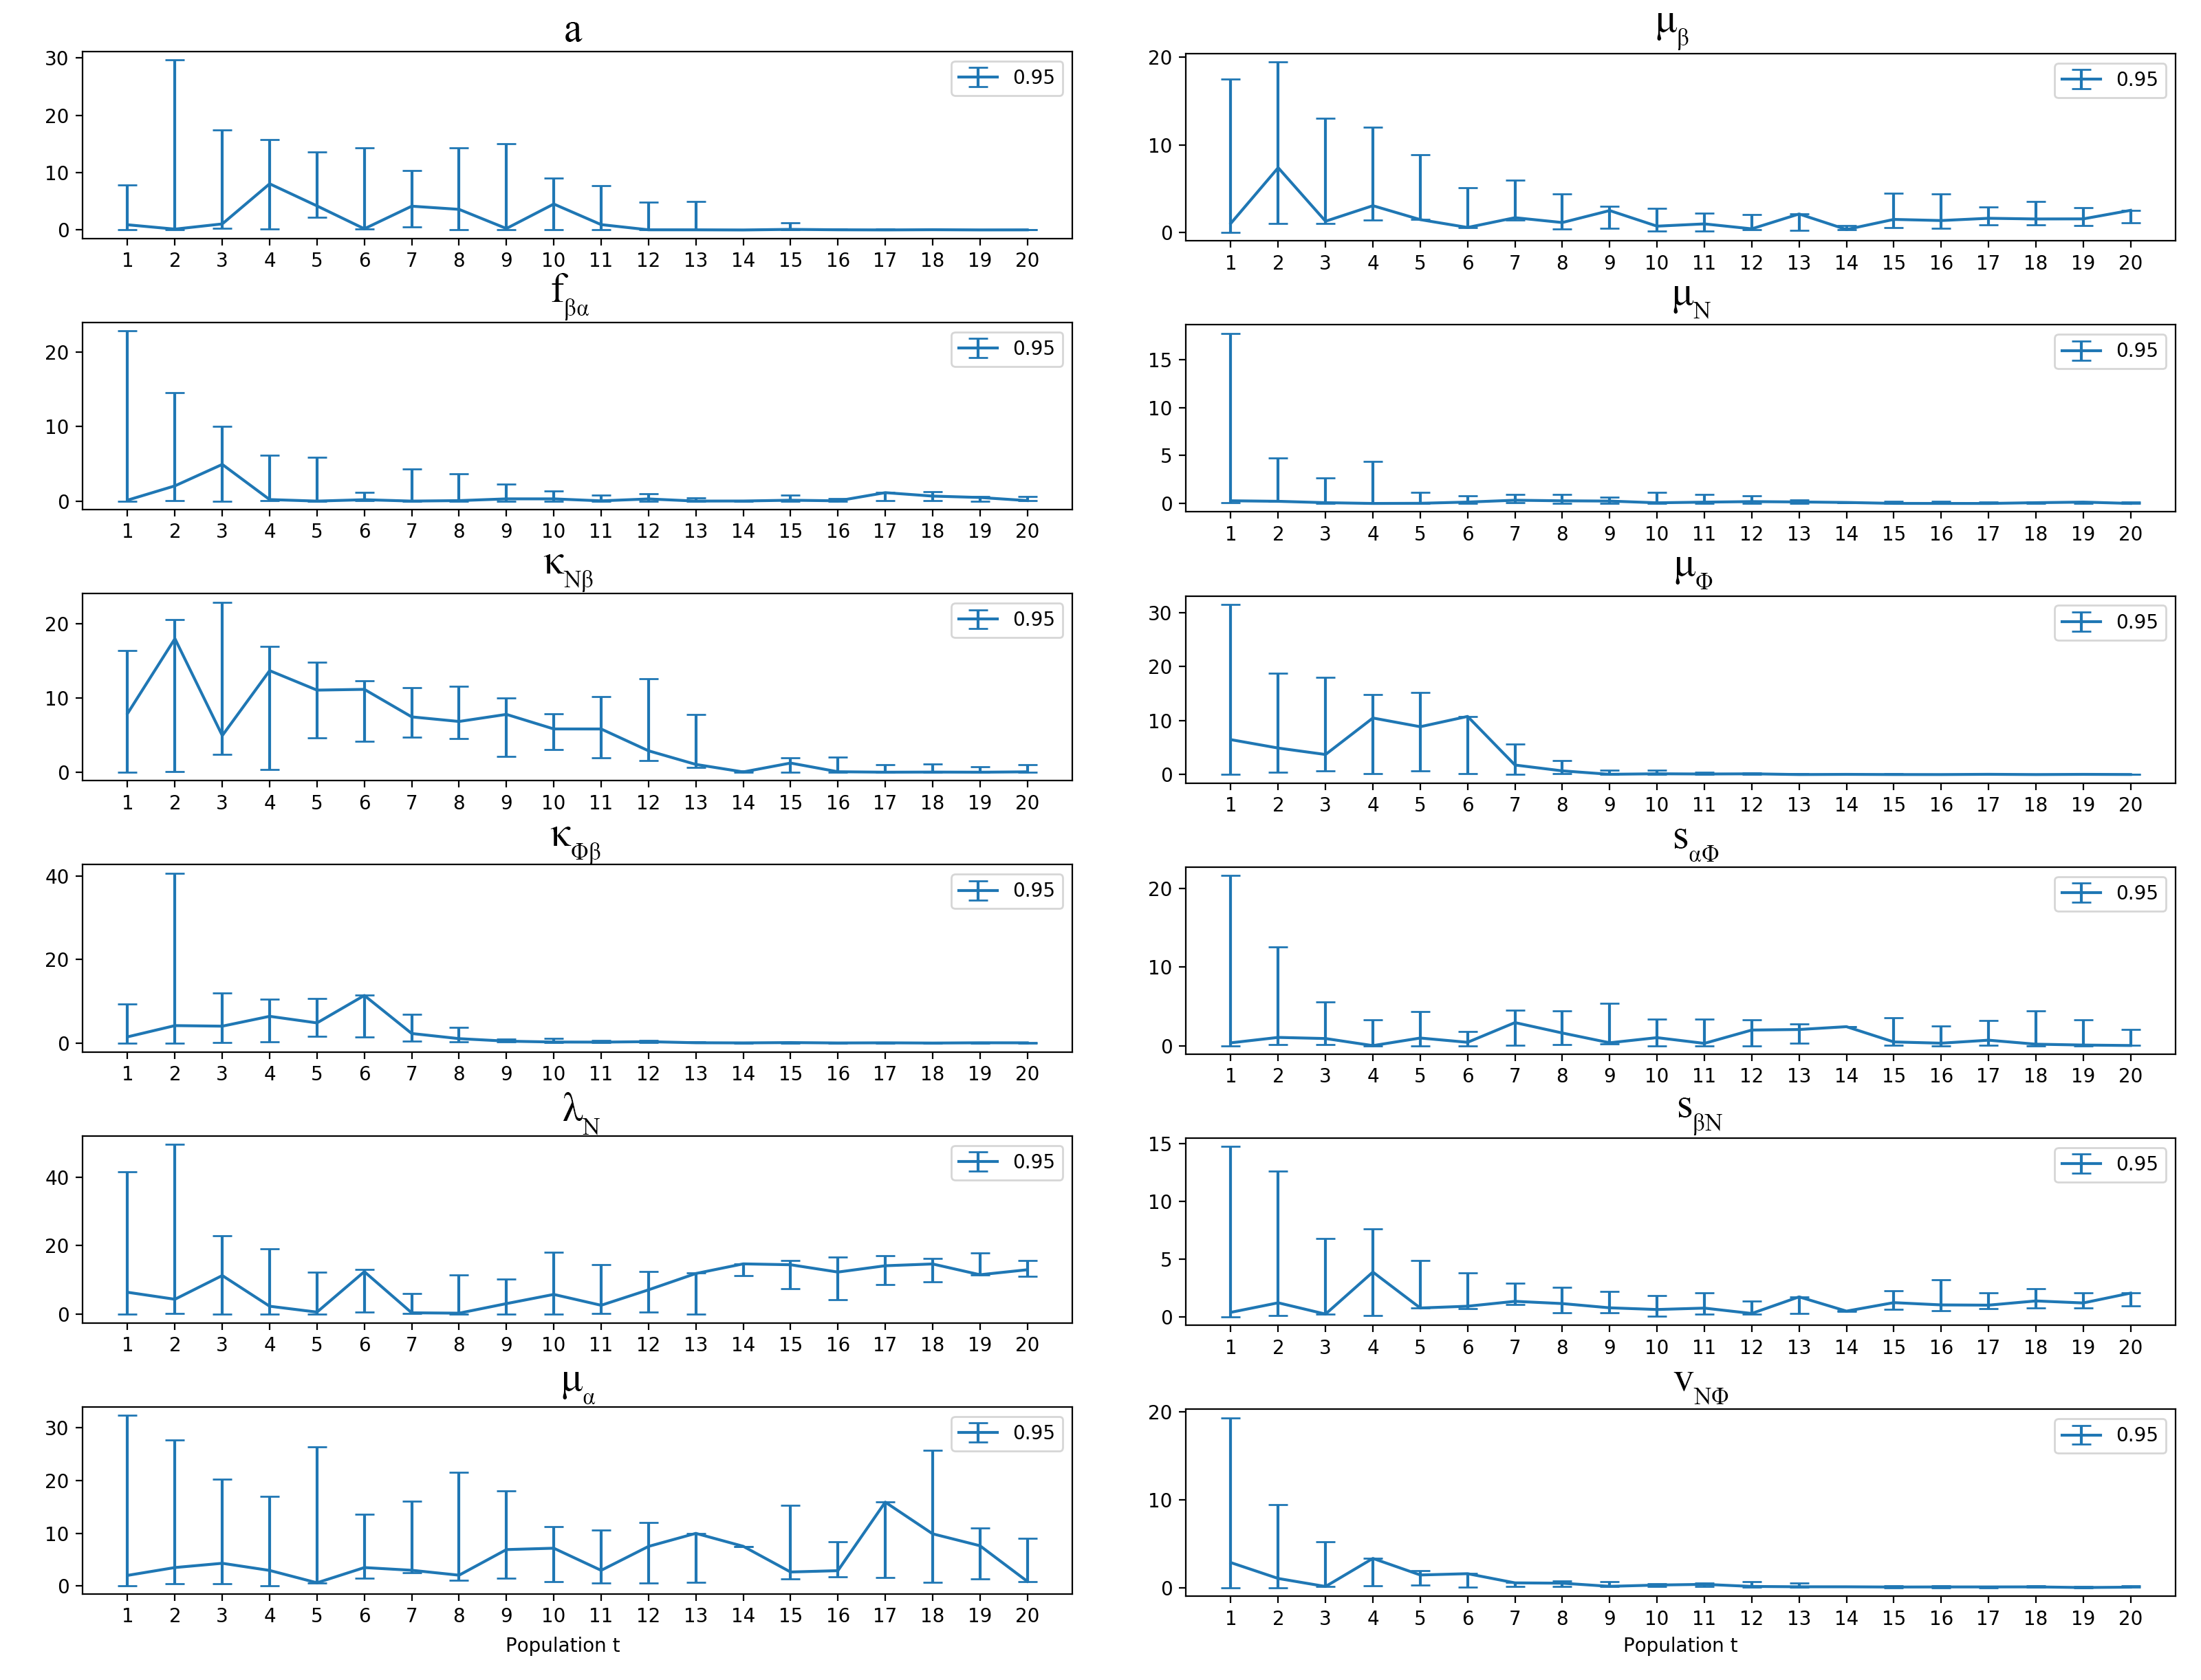
\includegraphics{fig/credible.png}}
    \end{center}
    \caption[Credible intervals of parameters in model 5]%
    {Credible intervals of parameters in model 5 across all generations}
    \label{fig:credible}
\end{figure}







